\documentclass[../../main.tex]{subfiles}
\begin{document}
\part{Analysis}
\chapter{Introduction}
For my project I will attempt to make a graphing software. Graphing software is incredibly important in Linear Algebra and a lot of maths taught in schools is to do with Linear Algebra. Linear Algebra also links to many other aspects of Maths and hence is very important to understand. My stakeholders will consist of teachers, who will use my software to show graphs of functions, and to students who will use it to practise their graph sketching or to help them with their homework. There are many graphing tools out there, some of them shown below, however they have many downsides. I hope to make a piece of software that has as much functionality as possible, while retaining simplicity and reducing the number of downsides to an absolute minimum.
\begin{figure}[H]
	\centering
	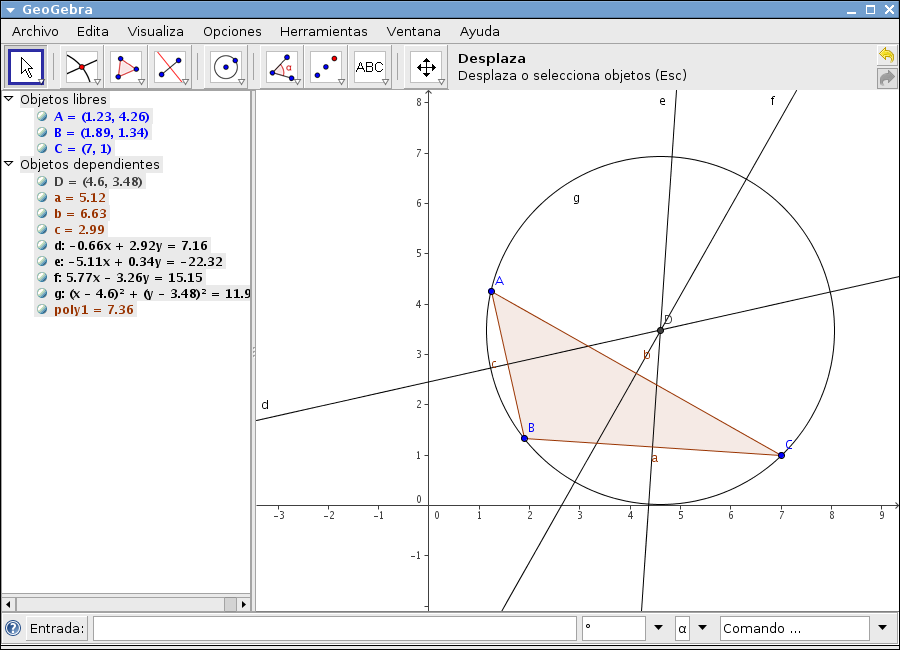
\includegraphics[width=.4\textwidth]{geogebraEx}
	\caption{GeoGebra}
\end{figure}
\begin{figure}[H]
	\centering
	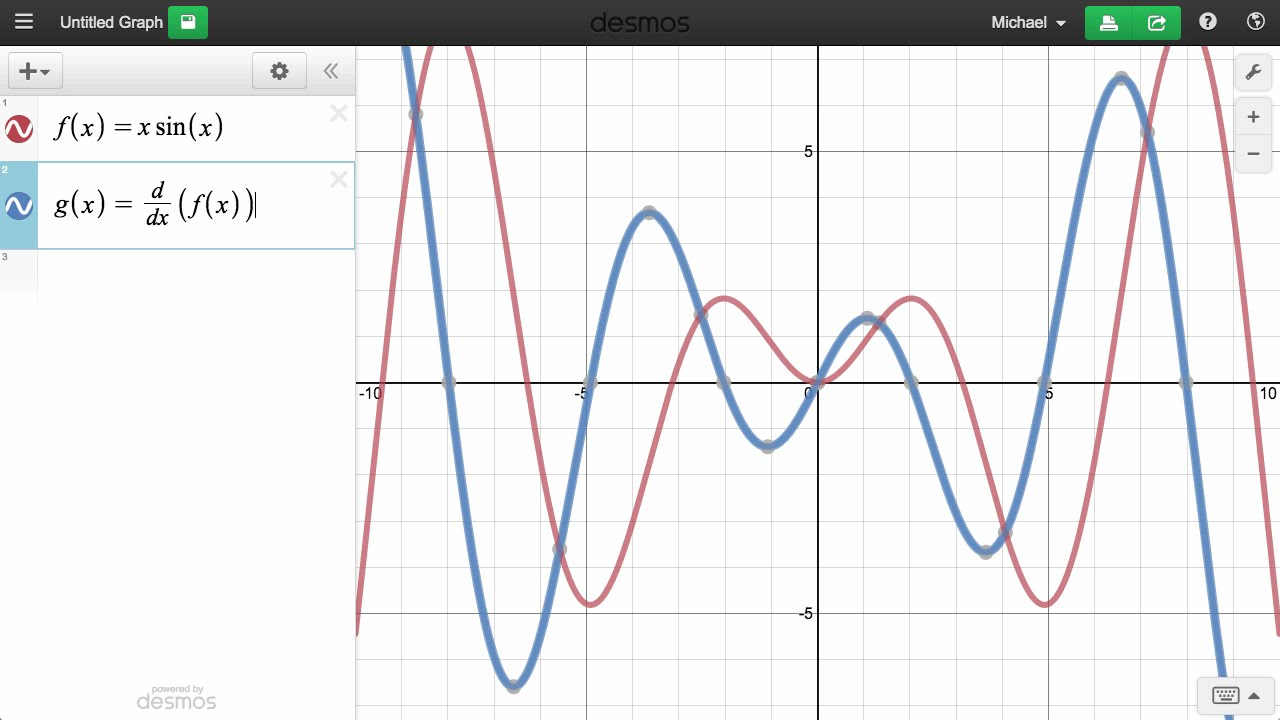
\includegraphics[width=.4\textwidth]{desmosEx}
	\caption{Desmos}
\end{figure}
\newpage
\end{document}